{\centering
{\scshape\LARGE Computer Vision and Image Processing M \par}
\vspace{1cm}
{\scshape\Large Report by Giada Martina Stivala - 0000820941 \par}
\vspace{1.5cm}
{\huge\bfseries Optical Character Recognition with Neural Networks\par}
\vspace{2cm} \par
}


\section*{Introduction}\label{introduction}

In this project we developed a system to address the problem of CAPTCHA
recognition. Most web services use CAPTCHAs to prevent automatic
navigation by robots and crawlers: an image with a series of letters and
numbers are shown to the user, who has to recognize them and write the
corresponding characters in a text box. CAPTCHAs can vary in complexity,
showing more or less letters, adding shifts and rotations as well
as noise and additional lines and points overlapping with the letters.

For our purposes, we chose to study and process only simple CAPTCHAs,
characterized by a low number of letters and digits, little degree of
overlapping and occlusion and little noise. Also, all of the letters are
written with a capital font and similar dimension, with the only
difference being the bold character. This choice reflected also the limited availability of hardware and computing power at our disposal.

Initially, the target of this project work was to perform character
recognition entirely with a neural network, trained on a large number of
labeled instances retrieved from the web. The task proved though to be
too complex for the available resources, thus imposing a simplification of the task.

Consequently, the complexity of CAPTCHAs was lowered, and the entire
project structure was reshaped into three different parts. The idea
behind this approach was to leverage on the OpenCV library, freely
available, to preprocess CAPTCHA images so to decrease the workload of
the neural network. We also considered to tackle the recognition task
with a \emph{divide et impera} approach, purposefully we extracted from
a single CAPTCHA image four sub-images containing the letters by
themselves, and the network was trained on single labeled letters.
Considering the learning process required to recognize a whole CAPTCHA
image with respect to the recognition of single characters, this
simplistic hypothesis turns out to be quite efficient.

In the first part, CAPTCHAs are loaded into memory and divided into
their four characters. Then, they are processed and organized in a set
for the neural network to use. In the second part, we build the neural
network model and complete the training; finally, a CAPTCHA image is
randomly picked and fed into the network for recognition. As the network
recognizes only alphanumeric characters, images are previously processed
to meet this requirement.

\vspace{1.5cm} \par
\section*{First task - image
processing}\label{first-task---image-processing}

In this section we address the image preprocessing aimed at simplifying
network training.

First, we draw a sample from the entire data set, and save it for later.
This is to test the network's predictive ability on unseen examples. To
do it, we use the Keras function \texttt{train\_test\_split}, which
automatically draws a random sample from the provided data set. The size
of the subset is 0.15 times the size of the entire dataset, which counts
9955 labeled CAPTCHAs. We then proceed to load the image and convert it
into grayscale. CAPTCHA images may be RGB, but colour does not provide
any additional information in terms of character recognition, thus we
prefer to remove it to simplify the learning process.

To apply the \emph{divide et impera} approach it is necessary to split
the image in its four letters, obtaining four sub-images. Thus, we need
to identify the contours of the characters, and then separate them into
four different images using their bounding box. During this step, the
main issue consisted in separating overlapped characters: in fact, the
bounding box happened to contain two characters at the same time as they
were detected as a single object. The problem was addressed with a
simple solution: if the width of the bounding rectangle was greater than
the height (we thresholded their ratio), the rectangle was divided in
two equal halves, each assigned to a character. As a result, some
characters appear to be missing edges or small pieces, but this was not
considered to be a flaw as it could help the network generalize better.
\begin{itemize}
\item Since we chose fairly simple CAPTCHAs with a low amount of noise, we
can assume that after turning the image into grayscale the histogram is
already bimodal. 
\item We can proceed with thresholding, leveraging in
particular on Otsu's automatic thresholding algorithm. In the OpenCV
\texttt{threshold} function, we select \texttt{THRESH\_BINARY\_INV} and
\texttt{TRESH\_OTSU}, obtaining the negative of the CAPTCHA. 
\begin{itemize}
	\item  Objects are assumed to be bright on a dark background.
\end{itemize}
\item We invoke \texttt{findContours},
selecting only the highest level of the contours hierarchy (the most
external contour, with the parameter \texttt{RETR\_EXTERNAL});
furthermore, since we have to use them to construct the bounding
rectangle, we select only the end points with
\texttt{CHAIN\_APPROX\_SIMPLE}. 
\item We feed the obtained contour into the
\texttt{boundingRect} function, obtaining a quadruple of points, the
first two being the top-left corner, followed by width and height of the
rectangle. The result is shown in Figure \ref{fig1-boundingboxCAPTCHA}.
\item To split the original image into four sub-images, first we
check if the obtained rectangle has valid values, possibly splitting the
bounding rectangle in two separate rectangles if two letters have been
recognized together. We also checked if, by any chance, the
\texttt{findContours} function recognized more than four objects,
discarding the whole CAPTCHA if this was the case. 
\item Finally, we applied
the bounding rectangles to the original grayscaled image, which was then
cut in four sub-images following those guidelines. We can see single letters and digits in Figure \ref{fig2-separatedCAPTCHA}.
\end{itemize}

Letters were separated from digits and saved separately, to train the network on separate classes.

\begin{figure}
	\centering
	\begin{minipage}{0.23\textwidth}
		\centering
		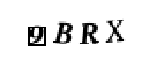
\includegraphics[width=1\textwidth]{boundingbox_1.png}
	\end{minipage}
	\begin{minipage}{0.23\textwidth}
		\centering
		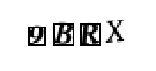
\includegraphics[width=1\textwidth]{boundingbox_2.png} 
		
	\end{minipage}
	\begin{minipage}{0.23\textwidth}
		\centering
		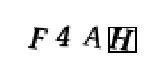
\includegraphics[width=1\textwidth]{boundingbox_3.png} 
		
	\end{minipage}
	\begin{minipage}{0.23\textwidth}
		\centering
		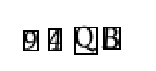
\includegraphics[width=1\textwidth]{boundingbox_4.png} 
	\end{minipage}
	\caption{CAPTCHAs with letters and numbers highlighted by a bounding box.}
	\label{fig1-boundingboxCAPTCHA}
\end{figure}

\begin{figure}
	\centering
	\begin{minipage}{0.20\textwidth}
		\centering
		
\includegraphics[width=0.2\textwidth]{letter-1.png}
	\end{minipage}
	\begin{minipage}{0.20\textwidth}
		\centering
		
\includegraphics[width=0.2\textwidth]{letter-2.png} 

	\end{minipage}
	\begin{minipage}{0.20\textwidth}
		\centering
		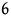
\includegraphics[width=0.2\textwidth]{letter-3.png} 
	
	\end{minipage}
	\begin{minipage}{0.20\textwidth}
		\centering
		
\includegraphics[width=0.2\textwidth]{letter-4.png} 
	\end{minipage}
	\caption{Letters after being cut from whole CAPTCHA images. It is possible to observe as some of them are skewed and missing little angles, or with additional object pieces coming from previously overlapped letters.}
	\label{fig2-separatedCAPTCHA}
\end{figure}

\vspace{1.5cm} \par
\section*{Second task - neural network}\label{second-task---neural-network}
In this section we discuss the architecture and performance of the neural network.

At the beginning of this stage we load the data we processed and add some final touches to start training. These include:
\begin{itemize}
	\item Choosing a set dimension for all the images, which will then be a parameter for the neural network;
	\item Creating a \texttt{numpy} array with an added dimension;
	\item Retrieving labels for testing;
	\item Normalize all images, from interval \texttt{[0, 255]} to interval \texttt{[0,1]}.
\end{itemize}

An additional, bigger partitioning of the training set is performed to obtain the validation set, used to calculate accuracy and loss during training. Finally, we instantiate a \texttt{Sequential} model for our convolutional neural network, adding as a first layer a \texttt{Conv2D} layer applying 20 (5x5) kernels on the 20x20x1 input tensor; the image is padded to obtain an output with the same dimension. Then we have a dropout layer with the \texttt{MaxPooling2D} operation, which gives a 10x10x20 tensor as an output. These two layers are added another time to the network, and followed by a fully-connected layer with activation function \texttt{relu}. Ultimately, the output layer is another fully-connected layer, having 32 neurons and \texttt{softmax} activation function.

With this configuration, the network trained on 29058 examples, and tested on a validation set of 9686 examples. The network performed well as we can see from the accuracy and loss graphs in Figure \ref{fig3-300-acc} and \ref{fig4-300-loss}.

\begin{figure}
	\centering
	\begin{minipage}{0.9\textwidth}
		\centering
		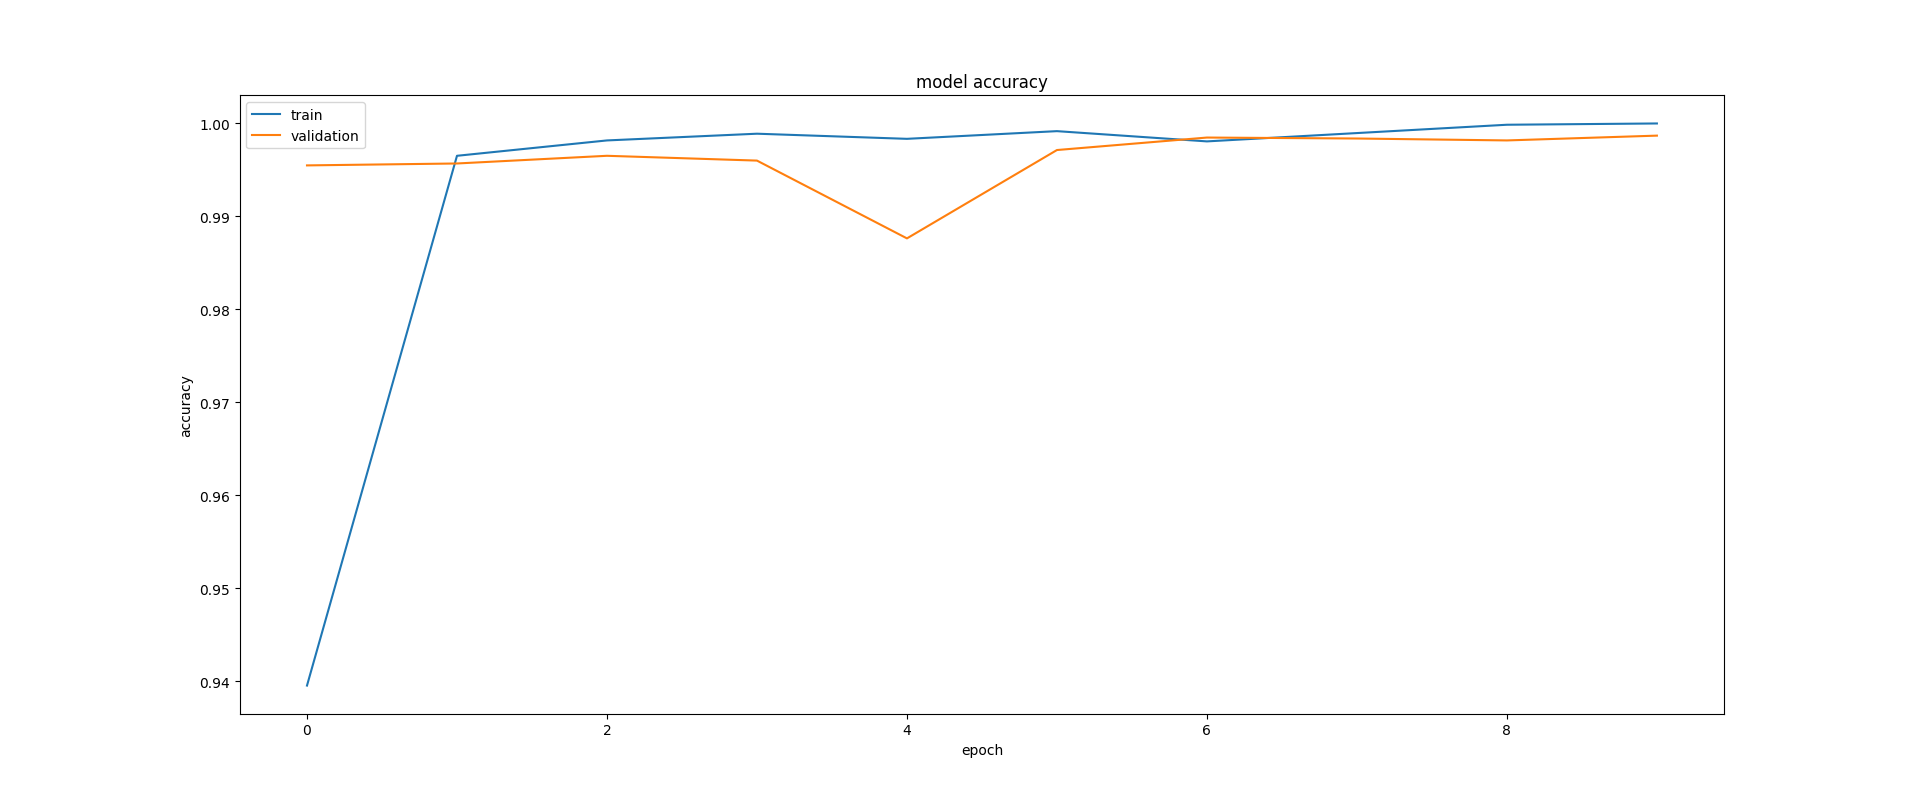
\includegraphics[width=1\textwidth]{300-acc_1.png}
	\end{minipage}
	\caption{Graph comparing accuracy of the network performing on training set and validation set.}
	\label{fig3-300-acc}
\end{figure}
\begin{figure}
	\centering
	\begin{minipage}{0.9\textwidth}
		\centering
		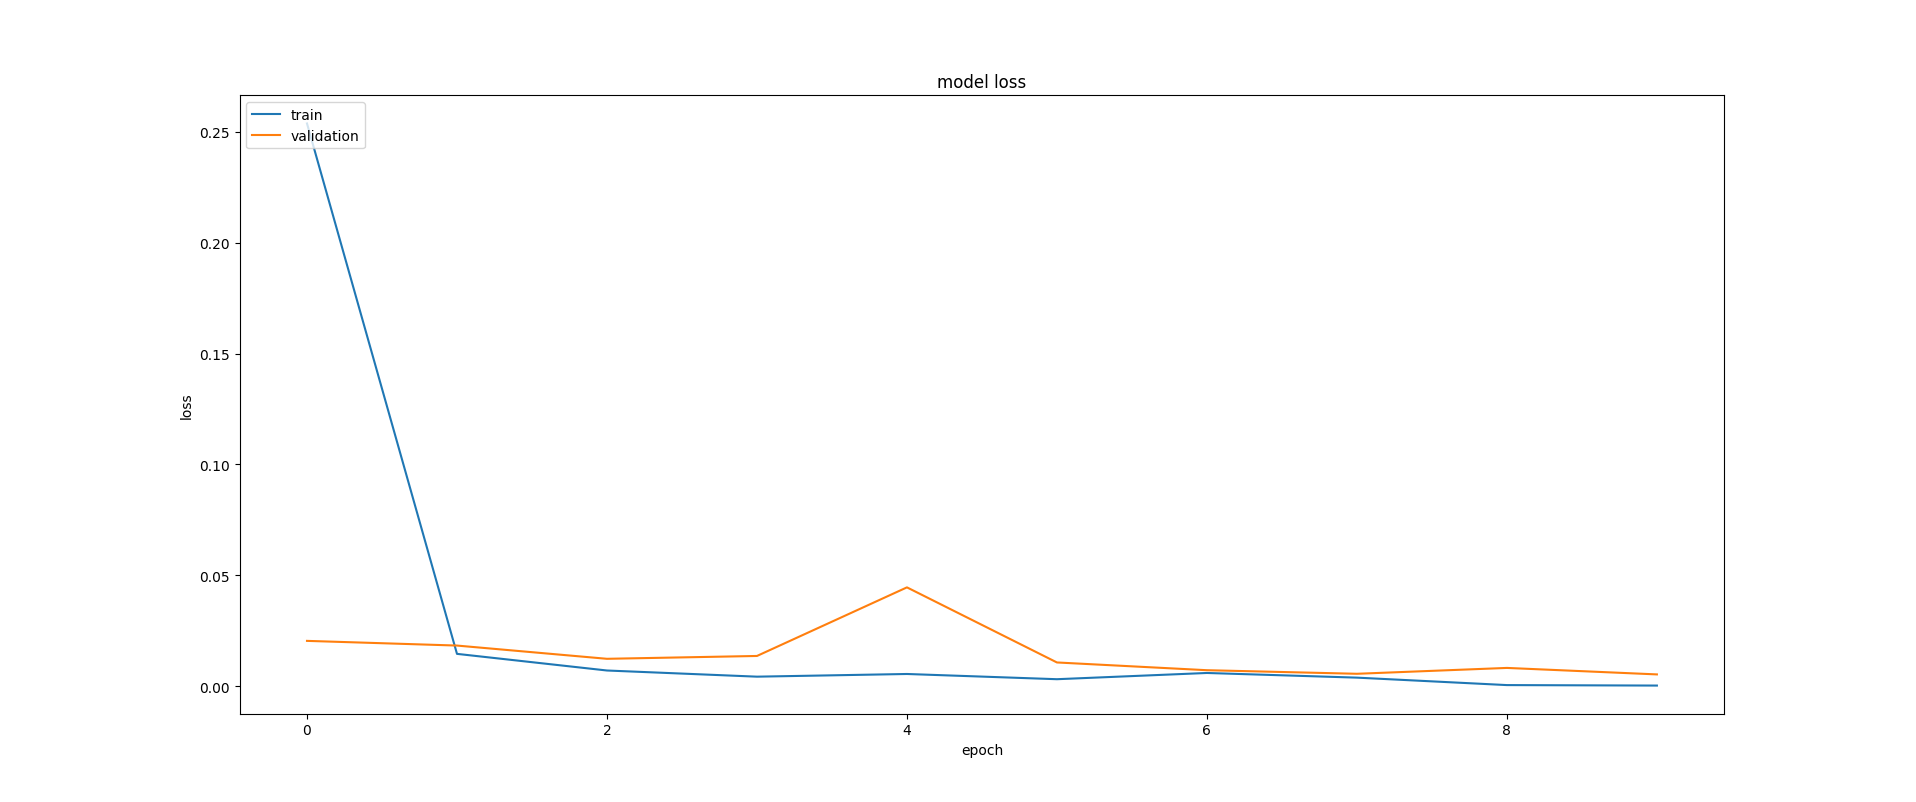
\includegraphics[width=1\textwidth]{300-loss_1.png} 
	\end{minipage}
	\caption{Graph comparing the loss of the network performing on training set and validation set.}
	\label{fig4-300-loss}
\end{figure}

To study the behaviour of the network and find some possible improvements, we tested two different aspects: first, we changed the structure of the network, adding more neurons in the hidden layer. Specifically, we moved from 300 to 500 neurons in the fully-connected layer, but the results showed a slight decrease of performance. In fact, even if the network seems to be slightly overfit (the accuracy on the training set being higher than the one on the validation set), adding more neurons strengthened this feature of the network, clearly indicating that we were moving in the wrong direction.

Secondly, we decided to add some more image preprocessing aimed at introducing more variations in the data set. We used the \texttt{ImageDataGenerator} available from Keras to insert random shifts both horizontally and vertically, together with rotations. The shifts could be up to 0.2 of the image dimension, and the rotation up to 15 degrees.

This new model performed quite differently from the original one: the accuracy on the training set dropped considerably, while accuracy on the validation set improved, showing a greater ability of the network to generalize. The same can be said for the loss function, as shown in Figure \ref{fig5-300dig-acc} and \ref{fig6-300dig-loss}. For testing purposes, we considered the performance of \texttt{ImageDataGenerator} also in the network with 500 hidden neurons. The results showed an improvement of performance, which was, nonetheless, poorer than the one obtained with 300 neurons.

\begin{figure}
	\centering
	\begin{minipage}{0.9\textwidth}
		\centering
		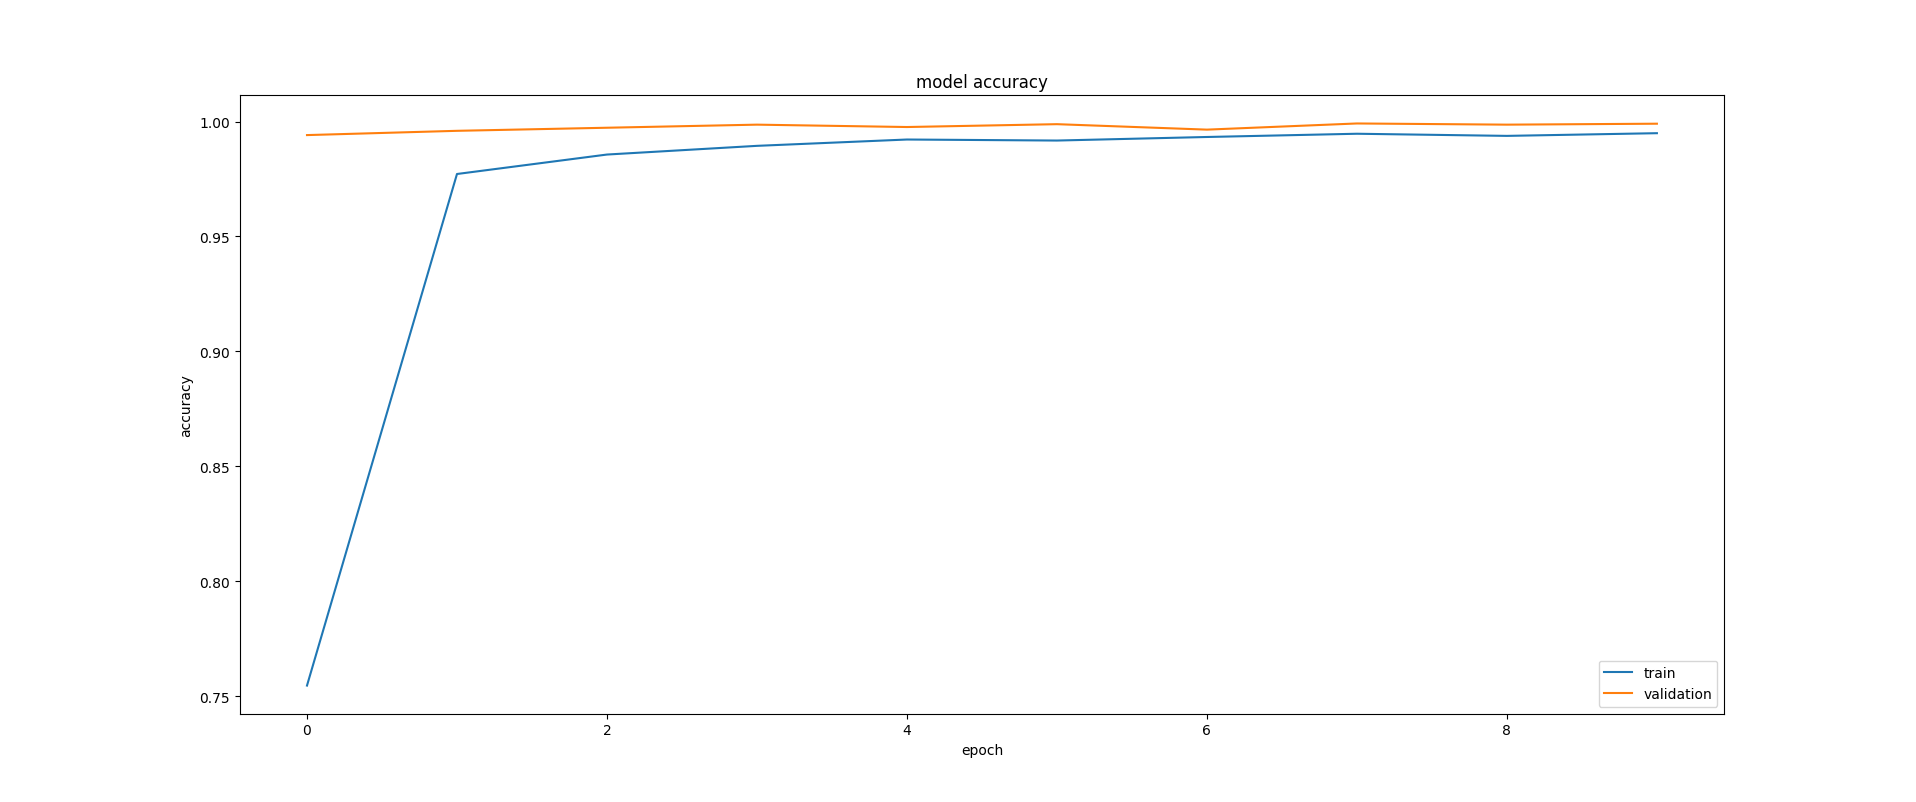
\includegraphics[width=1\textwidth]{300dig-acc_1.png}
	\end{minipage}
	\caption{Graph comparing accuracy of the network performing on training set and validation set, after the addition of an ImageDataGenerator.}
	\label{fig5-300dig-acc}
\end{figure}
\begin{figure}
	\centering
	\begin{minipage}{0.9\textwidth}
		\centering
		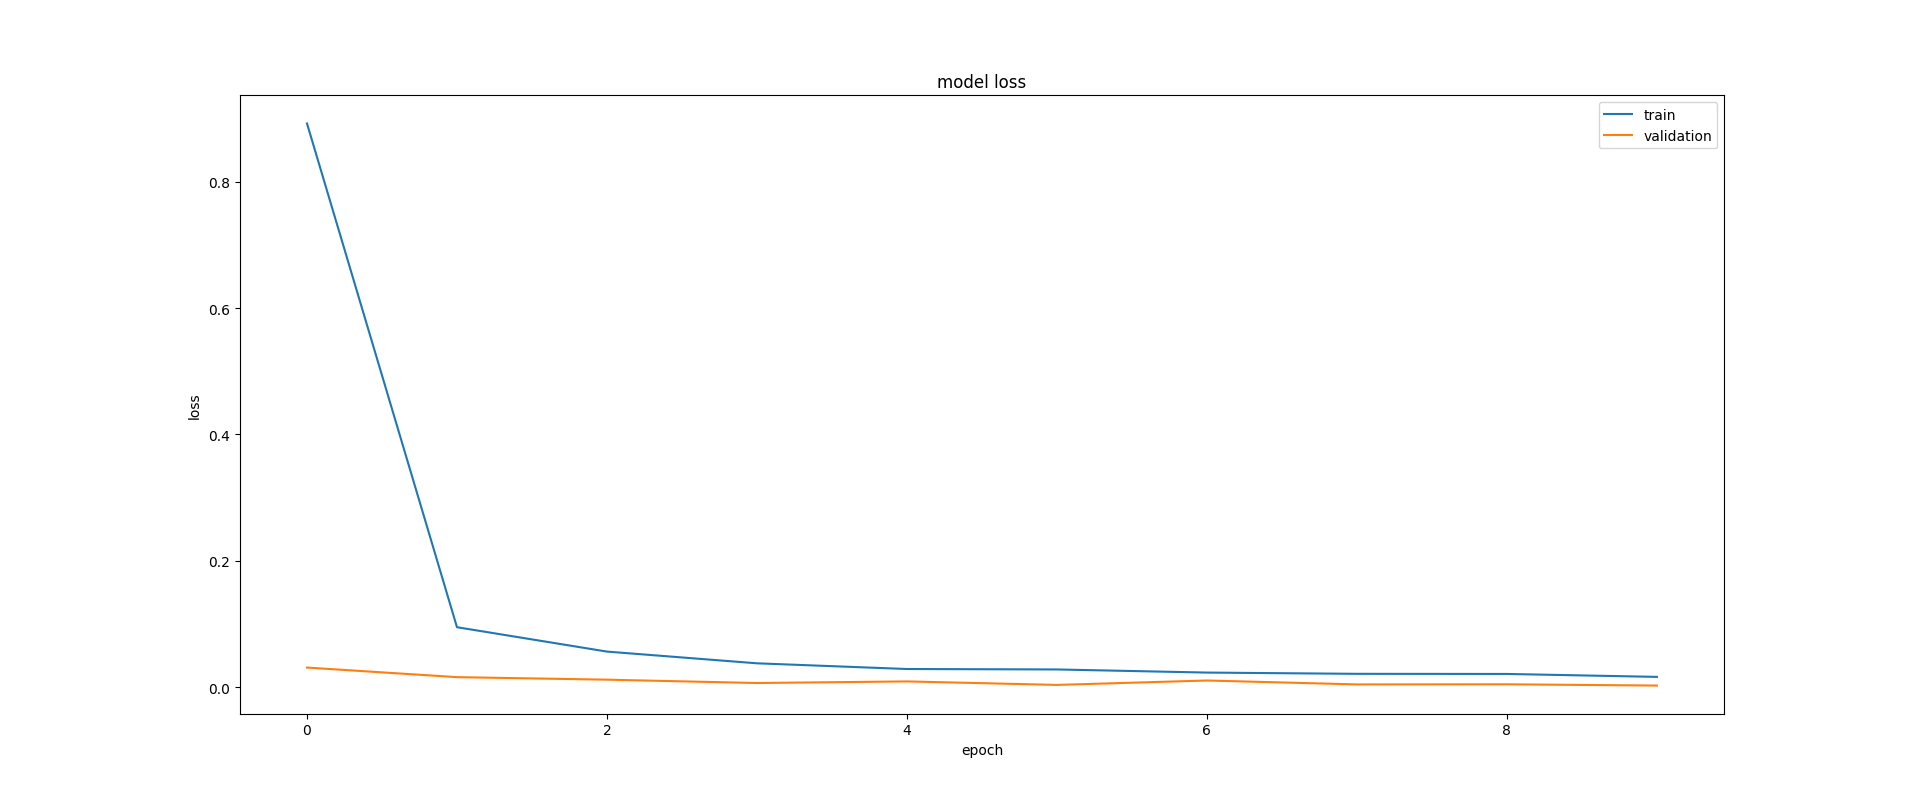
\includegraphics[width=1\textwidth]{300dig-loss_1.png} 
	\end{minipage}
	\caption{Graph comparing the loss of the network performing on training set and validation set, after the addition of an ImageDataGenerator.}
	\label{fig6-300dig-loss}
\end{figure}

We finally tested both networks on the unseen examples. They are 1490 randomly-selected CAPTCHAs, with four characters each, for an overall amount of 5960 predictions. We observed the following results:
\begin{itemize}
	\item The first network made 24 incorrect predictions on the whole dataset. Even if only a single letter was incorrect among the four composing a CAPTCHA, the entire prediction must be discarded.
	\item The second network made 29 incorrect predictions on the whole dataset. This goes against our previous considerations of a better performance.
\end{itemize}

In Figure \ref{fig7-wronglabels} are shown some of the incorrectly labeled images. We analysed the incorrectly labeled CAPCHAs for both networks and found out that:
\begin{itemize}
	\item For the first network, 13 over 24 incorrectly labeled characters were \textit{Q} letters which had inside their bounding rectangle some spurious element, probably due to incorrect binarization or cutting.
	\item We run the same check on the second network and found out a lower number of errors due to \textit{Q} incorrect labeling (11 over 29). A comparison of the two errors for this particular case shows a decrease of incorrect labeling from 54\% to 37\%. The remaining errors were "regular" wrong predictions with an even distribution.
\end{itemize}

\begin{figure}
	\centering
	\begin{minipage}{0.23\textwidth}
		\centering
		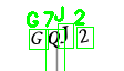
\includegraphics[width=1\textwidth]{wronglabel_1.png}
	\end{minipage}
	\begin{minipage}{0.23\textwidth}
		\centering
		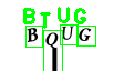
\includegraphics[width=1\textwidth]{wronglabel_2.png} 
		
	\end{minipage}
	\begin{minipage}{0.23\textwidth}
		\centering
		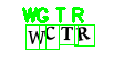
\includegraphics[width=1\textwidth]{wronglabel_3.png} 
		
	\end{minipage}
	\begin{minipage}{0.23\textwidth}
		\centering
		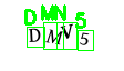
\includegraphics[width=1\textwidth]{wronglabel_4.png} 
	\end{minipage}
	\caption{Results of wrong predictions in unseen examples. We can notice, among them, some errors due to spurious objects in the image.}
	\label{fig7-wronglabels}
\end{figure}

\vspace{1.5cm} \par
\section*{Third task - predicting CAPTCHAs}\label{third-task---predicting-captchas}
The third step loads the unseen examples and the trained model, and calculates some statistics on performance. As the model predicts single letters, we repeated the process used in the first step to separate letters within CAPTCHAs.

\vspace{1.5cm} \par
\section*{Final considerations}\label{final-considerations}
We have presented a report for a project on Optical Character Recognition for the Computer Vision and Image Processing M university course. We have discussed possible different network architectures and their performance, evaluating them and identifying the best solution. We have also considered and employed ways to preprocess images, so as to simplify the training process and gain in efficiency.

This project makes use of OpenCV functions studied within the course as well as convolutional neural network training, which is not covered in the program. The choice of the topic is related to my own personal interest in Information Security, and I thought that "breaking CAPTCHAs" could be a project that fit both areas.

We focused on a simplified use case, in which the diversity between CAPTCHA characters is limited and there is little to no amount of added noise in the image. It could be a real use case only for web services with a low security risk, while CAPTCHAs employed in services as Amazon or Facebook are at another scale of difficulty.

Further developments and improvements could tackle more complex tasks; these involve using additional image preprocessing, to remove both noise and added lines or objects. Depending on the type of noise (usually both impulse and random noise), median and gaussian filtering can be employed. On the other side, to remove additional lines or objects we could use morphology transformations like opening and closing, available from the OpenCV library.